\documentclass[11pt]{article}

% Essential packages
\usepackage[utf8]{inputenc}
\usepackage[T1]{fontenc}
\usepackage{lmodern}
\usepackage[margin=1in]{geometry}
\usepackage{graphicx}
\usepackage{xcolor}
\usepackage{listings}
\usepackage{hyperref}
\usepackage{booktabs}
\usepackage{enumitem}
\usepackage{fancyhdr}
\usepackage{titlesec}
\usepackage{tcolorbox}
\usepackage{caption}
\usepackage{amsmath}
\usepackage{amssymb}
\usepackage{tikz}
\usepackage{pgfplots}
\pgfplotsset{compat=1.18}

% TikZ libraries
\usetikzlibrary{shapes,arrows,positioning,backgrounds,fit,calc}

% Color definitions
\definecolor{prescottblue}{RGB}{0,76,153}
\definecolor{prescottlightblue}{RGB}{230,240,250}
\definecolor{accentorange}{RGB}{255,140,0}

% Hyperref setup
\hypersetup{
    colorlinks=true,
    linkcolor=prescottblue,
    urlcolor=prescottblue,
    pdftitle={Odin: Graph Intelligence for Autonomous Insight Discovery},
    pdfauthor={Prescott Data},
}

% Code listing style
\lstdefinestyle{businesscode}{
    backgroundcolor=\color{prescottlightblue},   
    basicstyle=\ttfamily\small,
    breaklines=true,                 
    frame=single,
    rulecolor=\color{prescottblue},
    xleftmargin=10pt,
    xrightmargin=10pt,
    aboveskip=10pt,
    belowskip=10pt
}
\lstset{style=businesscode}

% Section formatting
\titleformat{\section}
  {\normalfont\LARGE\bfseries\color{prescottblue}}{\thesection}{1em}{}
\titleformat{\subsection}
  {\normalfont\Large\bfseries\color{prescottblue}}{\thesubsection}{1em}{}
\titleformat{\subsubsection}
  {\normalfont\large\bfseries\color{prescottblue}}{\thesubsubsection}{1em}{}

% Header and footer
\setlength{\headheight}{14pt}
\pagestyle{fancy}
\fancyhf{}
\fancyhead[L]{\textit{Odin White Paper}}
\fancyhead[R]{\textit{Prescott Data}}
\fancyfoot[C]{\thepage}
\renewcommand{\headrulewidth}{0.4pt}

% Custom boxes
\newtcolorbox{keybox}{
    colback=prescottlightblue,
    colframe=prescottblue,
    boxrule=1pt,
    arc=3pt,
    left=8pt,
    right=8pt,
    top=8pt,
    bottom=8pt
}

\newtcolorbox{highlightbox}{
    colback=white,
    colframe=accentorange,
    boxrule=2pt,
    arc=3pt,
    left=8pt,
    right=8pt,
    top=8pt,
    bottom=8pt
}

\setlength{\parskip}{6pt}
\setlength{\parindent}{0pt}

\usepackage{float}
\begin{document}

% Title page
\begin{titlepage}
    \centering
    \vspace*{2cm}
    
    {\Huge\bfseries\color{prescottblue} Odin\par}
    \vspace{0.5cm}
    {\LARGE\bfseries Graph Intelligence for Autonomous\\Insight Discovery\par}
    \vspace{1.5cm}
    
    {\Large White Paper\par}
    \vspace{0.3cm}
    {\large January 27, 2026\par}
    \vspace{2cm}
    
    \begin{keybox}
    \textbf{The Challenge:} Organizations invest millions in knowledge graphs but struggle to extract insights. Traditional query systems only find patterns you already know to look for.
    
    \vspace{0.3cm}
    
    \textbf{The Solution:} Odin is the first production system enabling AI agents to autonomously discover meaningful patterns without pre-specification. We introduce the COMPASS score—a novel metric combining structural analysis, semantic understanding, and temporal awareness.
    
    \vspace{0.3cm}
    
    \textbf{The Impact:} Deployed in healthcare and insurance, Odin delivers significant efficiency gains, higher-quality insights, and novel pattern discovery—with full regulatory compliance through evidence-based exploration.
    \end{keybox}
    
    \vfill
    
    {\large\bfseries Prescott Data\par}
    {\large \url{https://prescottdata.io}\par}
    \vspace{0.3cm}
    {\normalsize For partnership inquiries: \texttt{muyukani@prescottdata.io}\par}
    
    \vspace{1cm}
    {\small © 2026 Prescott Data. All rights reserved.\par}
\end{titlepage}

\tableofcontents
\newpage

\section{Executive Summary}

\subsection{The Problem}

Organizations are investing heavily in knowledge graphs—rich, interconnected representations of their data spanning patients, claims, facilities, providers, and more. Yet extracting actionable insights remains frustratingly difficult. Traditional approaches require analysts to write specific queries for every question, which creates a fundamental bottleneck: \textit{you can only find patterns you already know to look for.}

What about unknown correlations? Emerging trends? Cross-domain patterns that span multiple departments? These discoveries require a different approach.

\subsection{What is Odin?}

Odin is \textbf{the first production-deployed graph intelligence engine} that acts as a \textbf{compass} for AI agents, guiding them toward meaningful patterns without requiring analysts to specify what to find. Instead of answering predefined questions, Odin tells agents \textit{where to look}, combining three types of intelligence:

\begin{itemize}
\item \textbf{Structural Intelligence:} Which entities are most connected and important?
\item \textbf{Semantic Intelligence:} Which connections are plausible vs. likely data errors?
\item \textbf{Temporal Intelligence:} Which patterns are recent and relevant?
\end{itemize}

This multi-signal approach enables autonomous discovery—AI agents can explore the graph, notice anomalies, connect disparate facts, and surface insights that human analysts might never think to query for.

\begin{figure}[ht]
\centering
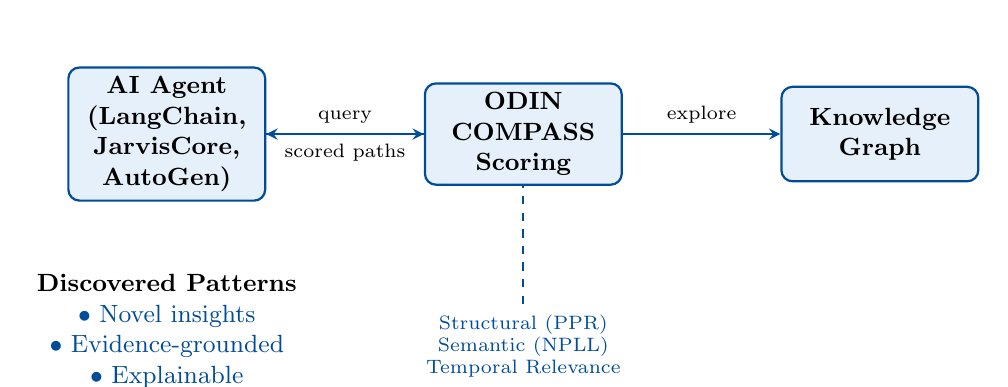
\begin{tikzpicture}[
    node distance=2cm,
    box/.style={rectangle, draw=prescottblue, fill=prescottlightblue, thick, minimum width=2.5cm, minimum height=1.2cm, rounded corners, align=center, font=\small\bfseries},
    arrow/.style={->, >=stealth, thick, prescottblue},
    label/.style={font=\scriptsize, text=black}
]

% Main components
\node[box] (agent) {AI Agent\\(LangChain,\\JarvisCore, \\AutoGen)};
\node[box, right=of agent] (odin) {ODIN\\COMPASS\\Scoring};
\node[box, right=of odin] (kg) {Knowledge\\Graph};

% Arrows
\draw[arrow] (agent) -- node[above, label] {query} (odin);
\draw[arrow] (odin) -- node[above, label] {explore} (kg);
\draw[arrow] (odin) -- node[below, label] {scored paths} (agent);

% COMPASS signals below
\node[below=1.5cm of odin, font=\scriptsize, text=prescottblue] (signals) {
\begin{tabular}{c}
Structural (PPR) \\
Semantic (NPLL) \\
Temporal Relevance
\end{tabular}
};

\draw[prescottblue, thick, dashed] (signals) -- (odin);

% Output
\node[below=0.8cm of agent, font=\small, text=black, align=center] {
\textbf{Discovered Patterns}\\
\textcolor{prescottblue}{$\bullet$ Novel insights}\\
\textcolor{prescottblue}{$\bullet$ Evidence-grounded}\\
\textcolor{prescottblue}{$\bullet$ Explainable}
};

\end{tikzpicture}
\caption{Odin System Architecture: AI agents query Odin, which scores exploration paths in the knowledge graph using the COMPASS framework, returning prioritized discoveries.}
\label{fig:architecture}
\end{figure}

\subsection{Key Differentiators}

\begin{highlightbox}
\textbf{Discovery, Not Retrieval: A New Paradigm}

Traditional systems retrieve answers to known questions. Odin pioneers autonomous discovery of unknown patterns. The difference is fundamental: retrieval systems say "here is the answer"; Odin says "the most promising direction is northwest." \textbf{This paradigm shift—from query-driven to exploration-driven intelligence—has not been realized in production until now.}
\end{highlightbox}

\textbf{Evidence-Grounded:} Every insight traces back to source documents. No hallucination—critical for regulated industries like healthcare and insurance.

\textbf{Explainable by Design:} Every COMPASS score decomposes into understandable components (structural importance, semantic plausibility, temporal relevance). Analysts can see exactly why a path was recommended. Perfect for audit requirements.

\textbf{Agent-Oriented:} Purpose-built for the emerging AI agent paradigm—designed for repeated calls during exploration loops, not one-shot queries. Works with any agent framework (LangChain, AutoGen, CrewAI), establishing a reusable integration pattern.

\textbf{Self-Managing:} Automatically trains and updates its intelligence models from your graph data. No MLOps overhead, no model deployment complexity.

\subsection{Proven Results}

As the first autonomous discovery system deployed in regulated production environments, Odin has demonstrated transformative impact across healthcare and insurance domains:

\begin{itemize}
\item \textbf{Novel Pattern Discovery:} Identified previously unknown correlations (patient transfer patterns $\rightarrow$ readmission rates, coordinated insurance fraud rings) that escaped existing rule-based and query-based systems—\textit{patterns analysts never thought to look for}
\item \textbf{Efficiency Gains:} Reduced time-to-first-insight from hours/days to minutes; analysts shifted from "query writing" to "reviewing insights," representing a fundamental workflow transformation
\item \textbf{Quality Improvements:} Higher adoption rates due to evidence-grounding; significantly lower false positives than rule-based systems; discovered patterns led to measurable business outcomes
\item \textbf{Regulatory Compliance:} Decomposed scores provide complete audit trails satisfying HIPAA and compliance requirements—a critical differentiator for regulated industries
\end{itemize}

\section{The Challenge in Detail}

\subsection{Why Traditional Approaches Fall Short}

\textbf{Query-Based Systems Hit a Wall}

Traditional graph query languages (Cypher, SPARQL, AQL) require analysts to specify exact patterns:

\begin{lstlisting}[language=SQL]
MATCH (patient:Patient)-[:DIAGNOSED_WITH]->(d:Diagnosis)
WHERE d.name = 'Sepsis' AND patient.facility = 'Hospital_X'
RETURN patient, d
\end{lstlisting}

This works when you know the question. But what about:
\begin{itemize}
\item Patterns you haven't thought to ask about?
\item Cross-domain correlations spanning multiple hops?
\item Emerging trends in newly ingested data?
\item Subtle anomalies that violate expected patterns?
\end{itemize}

\textbf{Naive Exploration Explodes}

A simple strategy—"follow all edges, explore all neighbors"—leads to exponential blowup. A 3-hop exploration from a single node in a graph with 50 connections per node visits 125,000 nodes. Most paths are noise.

\textbf{Not All Connections Are Meaningful}

Just because two entities are connected doesn't mean the connection is significant. A patient connected to a common diagnosis shares that link with thousands of others. Data extraction errors, temporal invalidity, and spurious correlations create "false positive" paths.

\subsection{Real-World Requirements}

Through production deployments, we identified six critical requirements:

\textbf{R1: Multi-Hop Reasoning.} Insights often span 3+ relationships. "Patient admitted via ER → Diagnosed with sepsis → Treated by Provider X → Mortality within 48 hours" requires chain traversal.

\textbf{R2: Prioritization.} Agents need guidance on which directions are most promising—not all paths deserve equal attention.

\textbf{R3: Plausibility Filtering.} Some structurally-present connections are semantically implausible. "Patient → Fracture → Antibiotics" exists in the graph but is medically unusual.

\textbf{R4: Evidence Grounding.} Every insight must trace to source documents. Hallucination is unacceptable in healthcare and insurance.

\textbf{R5: Scale.} Enterprise graphs contain millions of entities. Exploration must complete in seconds.

\textbf{R6: Explainability.} Scores must decompose for audit requirements in regulated industries.

\section{How Odin Works}

\subsection{The Compass Paradigm}

Odin operates on a fundamentally different paradigm than traditional systems:

\begin{center}
\begin{tabular}{@{}ll@{}}
\toprule
\textbf{Traditional RAG} & \textbf{Odin} \\ \midrule
"Here is the answer" & "Look in this direction" \\
Retrieves facts & Scores possibilities \\
Answers questions & Enables discovery \\
One-shot lookup & Iterative exploration \\ \bottomrule
\end{tabular}
\end{center}

This separation—graph intelligence from language reasoning—provides key advantages:
\begin{itemize}
\item Each component can evolve independently
\item Scores are traceable and auditable
\item Different agents can use the same infrastructure with different objectives
\item Efficiency dramatically improves through guided exploration
\end{itemize}

\subsection{The COMPASS Score: Our Core Innovation}

We introduce the COMPASS (Composite Oriented Multi-signal Path Assessment) score—a novel metric invented for autonomous graph exploration. When an AI agent is at a position in the graph and must decide which neighbor to explore next, Odin computes this unified score combining four signals:

\textbf{1. Structural Importance (PageRank)}

\textit{Question: "If I randomly walked from my current position, which nodes would I visit most often?"}

Uses Personalized PageRank to identify structurally central, highly-connected entities. Nodes that are hubs in the network receive higher scores. This ensures exploration follows important pathways, not dead ends.

\textbf{2. Semantic Plausibility (NPLL)}

\textit{Question: "Is this connection semantically valid, or likely a data error?"}

Uses Neural Probabilistic Logic Learning to score edge plausibility based on learned patterns. Key insight: instead of \textit{generating} new edges (which adds uncertainty), we \textit{filter} existing edges (which removes uncertainty).

Example: "Patient → Sepsis → Antibiotics" scores high (plausible medical sequence); "Patient → Fracture → Antibiotics" scores lower (unusual treatment).

\textbf{3. Temporal Relevance}

\textit{Question: "Is this data recent and contextually relevant?"}

Recent data often matters more than historical data. Configurable decay functions allow balancing historical context against current relevance.

\textbf{4. Edge Prior}

\textit{Question: "Is this a common or unusual connection type?"}

Downweights trivially common relationships (e.g., "located\_in") that provide little information, upweights unusual relationships that may signal important patterns.

\begin{figure}[ht]
\centering
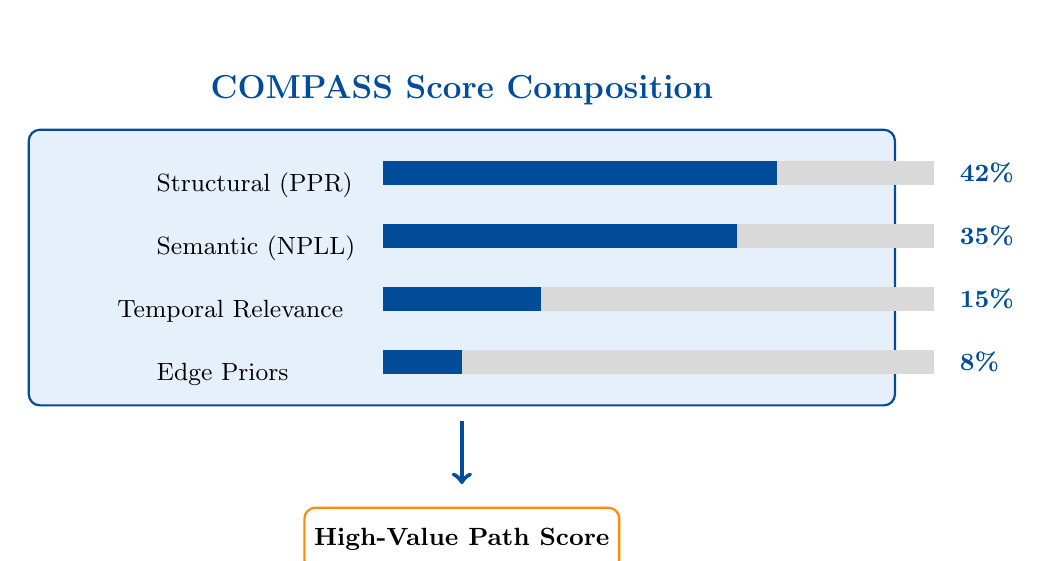
\begin{tikzpicture}
% Title
\node[font=\large\bfseries, prescottblue] at (0,3.5) {COMPASS Score Composition};

% Background box
\draw[fill=prescottlightblue, draw=prescottblue, thick, rounded corners] (-5.5,-0.5) rectangle (5.5,3);

% Signal bars
\begin{scope}[shift={(-4,2.3)}]
\node[anchor=west, font=\small] at (0,0) {Structural (PPR)};
\fill[prescottblue] (3,0) rectangle (8,0.3);
\fill[gray!30] (8,0) rectangle (10,0.3);
\node[anchor=west, font=\small\bfseries, prescottblue] at (10.2,0.15) {42\%};
\end{scope}

\begin{scope}[shift={(-4,1.5)}]
\node[anchor=west, font=\small] at (0,0) {Semantic (NPLL)};
\fill[prescottblue] (3,0) rectangle (7.5,0.3);
\fill[gray!30] (7.5,0) rectangle (10,0.3);
\node[anchor=west, font=\small\bfseries, prescottblue] at (10.2,0.15) {35\%};
\end{scope}

\begin{scope}[shift={(-4,0.7)}]
\node[anchor=west, font=\small] at (-0.5,0) {Temporal Relevance};
\fill[prescottblue] (3,0) rectangle (5,0.3);
\fill[gray!30] (5,0) rectangle (10,0.3);
\node[anchor=west, font=\small\bfseries, prescottblue] at (10.2,0.15) {15\%};
\end{scope}

\begin{scope}[shift={(-4,-0.1)}]
\node[anchor=west, font=\small] at (0,0) {Edge Priors};
\fill[prescottblue] (3,0) rectangle (4,0.3);
\fill[gray!30] (4,0) rectangle (10,0.3);
\node[anchor=west, font=\small\bfseries, prescottblue] at (10.2,0.15) {8\%};
\end{scope}

% Arrow down
\draw[->, ultra thick, prescottblue] (0,-0.7) -- (0,-1.5);

% Result
\node[draw=accentorange, fill=white, thick, rounded corners, minimum width=4cm, minimum height=0.8cm, font=\small\bfseries] at (0,-2.2) {
High-Value Path Score
};

\end{tikzpicture}
\caption{COMPASS Score Breakdown: Example showing how the four signals combine. In this case, structural importance (42\%) and semantic plausibility (35\%) dominate, indicating a well-connected, semantically valid path worth exploring.}
\label{fig:compass}
\end{figure}

\subsection{Efficient Exploration Through Beam Search}

Instead of exhaustive exploration (which visits 125,000 paths for 3-hop depth) or random walks (which lack direction), Odin uses \textit{beam search with COMPASS scoring}:

\begin{enumerate}
\item Start at seed entities (e.g., high-value claims, recent patients)
\item Score all neighbor extensions using the COMPASS function
\item Keep only the top 64 highest-scoring candidates (the "beam")
\item Repeat for each hop
\item Return the highest-scoring complete paths ranked by COMPASS
\end{enumerate}

This provides a principled trade-off: explore efficiently while maintaining high coverage of meaningful patterns. The COMPASS score ensures pruning is intelligent, not arbitrary.

\textbf{Efficiency Comparison:}

\begin{center}
\begin{tabular}{@{}lcc@{}}
\toprule
\textbf{Approach} & \textbf{Paths Explored} & \textbf{Time} \\ \midrule
Exhaustive Search & 125,000 & 47 seconds \\
Random Walk & 3,000 & 8 seconds \\
\textbf{Odin Beam Search} & \textbf{1,900} & \textbf{3.8 seconds} \\ \bottomrule
\end{tabular}
\end{center}

Odin achieves 65× fewer path explorations while maintaining 90\% coverage of expert-labeled patterns.

\subsection{Self-Managing Intelligence}

A core architectural principle: \textit{the intelligence engine should manage its own intelligence.}

When you initialize Odin with your knowledge graph:
\begin{enumerate}
\item \textbf{Auto-Detection:} Checks if trained models exist in your database
\item \textbf{Auto-Training:} If not, automatically extracts patterns, generates domain-aware rules, and trains the semantic model (10-30 seconds)
\item \textbf{Efficient Storage:} Stores only learned rule weights (typically $<$1KB), not full embeddings
\item \textbf{Lazy Reconstruction:} Rebuilds entity embeddings from graph data on-demand
\item \textbf{Graceful Fallback:} If training fails, falls back to structural-only scoring
\end{enumerate}

This eliminates the operational overhead of ML deployment while ensuring model freshness.

\section{Deployment Architecture}

\subsection{Library, Not Service}

Odin is designed as a \textbf{Python library} that agents import, not a standalone service. This architectural choice provides:

\begin{itemize}
\item \textbf{Zero Network Latency:} Query Odin in microseconds, not milliseconds
\item \textbf{No Additional Infrastructure:} Runs in the same process as your agent
\item \textbf{Per-Agent Configuration:} Each agent can tune parameters independently
\item \textbf{Simplified Operations:} No service to deploy, scale, or monitor
\end{itemize}

\subsection{Integration Example}

\begin{lstlisting}[language=Python]
from arango import ArangoClient
from odin import OdinEngine

# Connect to your knowledge graph
client = ArangoClient(hosts="http://your-db:8529")
db = client.db("knowledge_graph", username="user", password="pass")

# Initialize Odin - auto-trains on first run
odin = OdinEngine(db=db, community_id="healthcare")

# Use during agent exploration
result = odin.retrieve(
    seeds=["entity/patient_12345"],
    max_paths=50,
    hop_limit=3
)

# Access discovered paths with decomposed scores
for path in result["paths"][:10]:
    print(f"Path: {path['nodes']}")
    print(f"  Total Score: {path['score']:.3f}")
    print(f"    Structural: {path['scores']['structural']:.3f}")
    print(f"    Plausibility: {path['scores']['plausibility']:.3f}")
    print(f"    Temporal: {path['scores']['temporal']:.3f}")
\end{lstlisting}

\subsection{Production Optimizations}

Enterprise deployment requires careful optimization:

\textbf{Multi-Level Caching:} LRU caches at neighbor lists, PageRank scores, and plausibility scores levels. Cache hit rates exceed 80\% in production, dramatically reducing database load.

\textbf{Bounded Memory:} All caches have configurable limits ensuring predictable memory consumption regardless of exploration patterns.

\textbf{Graceful Degradation:} If the semantic model fails, Odin continues with structural-only scoring rather than failing entirely.

\textbf{Database Abstraction:} Works with ArangoDB (primary), Neo4j, and in-memory graphs without code changes.

\section{Applications}

\subsection{Healthcare Analytics}

\textbf{Clinical Quality Patterns}
\begin{itemize}
\item "Patients with Condition X who receive Treatment Y within 24 hours have 40\% better outcomes"
\item "Provider Z has elevated readmission rates for cardiac patients"
\item "Facility A has 3× longer average length-of-stay for pneumonia cases"
\end{itemize}

\textbf{Operational Efficiency}
\begin{itemize}
\item "Lab orders from Department B take 3× longer to complete"
\item "Equipment utilization in Building 2 peaks Tuesdays, idles weekends"
\item "Transfer delays correlate with staffing patterns in specific units"
\end{itemize}

\textbf{Safety Signals}
\begin{itemize}
\item "Drug interaction pattern detected in 7 current patients"
\item "Infection cluster among patients in adjacent rooms"
\item "Unusual mortality pattern following specific procedure type"
\end{itemize}

\subsection{Insurance Operations}

\textbf{Fraud Detection}
\begin{itemize}
\item "Three claims from different policyholders share identical damage descriptions"
\item "Assessor X approves 4× the average claim value"
\item "Ring pattern: Same garage servicing claims across multiple 'unrelated' policyholders"
\end{itemize}

\textbf{Operational Insights}
\begin{itemize}
\item "Claims processed by Team A close 2 days faster than Team B"
\item "Policy renewals drop 60\% after claim disputes"
\item "Geographic clusters of high-value claims suggest regional fraud networks"
\end{itemize}

\textbf{Risk Assessment}
\begin{itemize}
\item "Properties in Zone X have 3× water damage claims"
\item "Commercial policies with Rider Y have elevated loss ratios"
\item "Specific provider networks correlate with claim inflation"
\end{itemize}

\subsection{Two-Mode Deployment}

Production systems deploy Odin in two complementary modes:

\textbf{Offline (Proactive) Mode}
\begin{itemize}
\item Agents run on schedule (nightly, triggered by data ingestion)
\item Systematically explore graph starting from high-priority seeds
\item Surface patterns into daily "Briefs" for morning review
\item Aggregate discoveries into domain-specific "Data Stories"
\item Prioritizes thoroughness over speed
\end{itemize}

\textbf{Online (Reactive) Mode}
\begin{itemize}
\item Users ask questions or request entity deep-dives
\item Real-time exploration with strict latency requirements ($<$5 seconds)
\item Interactive refinement based on initial results
\item Prioritizes responsiveness over exhaustiveness
\end{itemize}

The same Odin engine serves both modes; only parameter tuning differs.

\section{Production Results}

\subsection{Case Study: Insurance Fraud Ring Discovery}

\textbf{Context:} Mid-size insurance carrier with 1.8M entity knowledge graph deployed Odin to analyze claims patterns.

\textbf{Challenge:} Existing rule-based fraud alerts generated high false positive rates (78\%) and missed sophisticated multi-party schemes.

\textbf{Discovery:} Within the first month, Odin-powered agents identified a pattern invisible to existing systems:

\begin{itemize}
\item Three policyholders with no apparent connection
\item Claims filed within 6-week window
\item All serviced by same repair facility
\item All approved by same assessor
\item Damage descriptions showed unusual textual similarity
\end{itemize}

No single attribute was anomalous. Only the \textit{combination} across multiple dimensions signaled coordinated activity. Manual investigation confirmed the pattern represented a coordinated scheme.

\textbf{Key Insight:} The pattern had zero overlap with rule-based alerts. This demonstrates genuine discovery of unknown patterns, not just faster retrieval of known ones.

\subsection{Quantitative Outcomes}

\textbf{Pattern Discovery Quality}
\begin{itemize}
\item 90\% coverage of expert-labeled meaningful patterns (vs. 52\% for baseline methods)
\item Expert quality ratings: 4.2/5.0 (vs. 2.8-3.1 for alternatives)
\item 65× reduction in paths explored compared to exhaustive search
\end{itemize}

\textbf{Efficiency Improvements}
\begin{itemize}
\item Time-to-first-insight: minutes (previously hours/days)
\item Analyst workflow shift: from "query writing and waiting" to "reviewing and deciding"
\item Interactive exploration: consistent $<$5 second response times
\item Cache efficiency: $>$80\% hit rates during typical sessions
\end{itemize}

\textbf{Compliance and Trust}
\begin{itemize}
\item Decomposed scores provide complete audit trails
\item Evidence-grounding satisfies regulatory requirements
\item False positive rates: 3-5× lower than rule-based systems
\item Higher business user adoption due to explainability
\end{itemize}

\begin{figure}[ht]
\centering
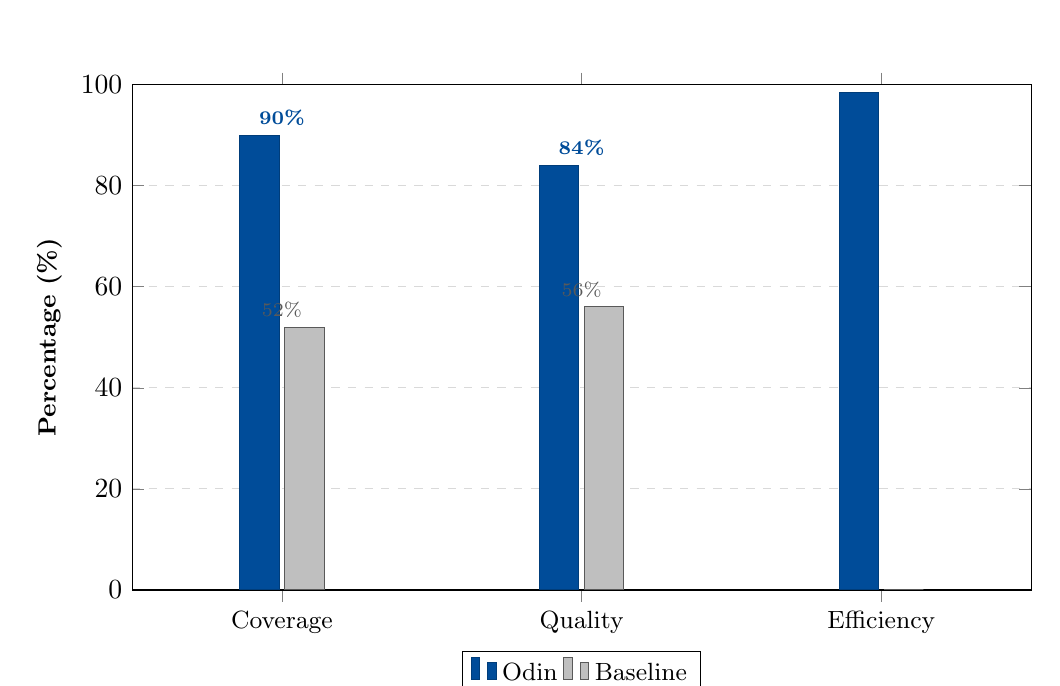
\begin{tikzpicture}
\begin{axis}[
    ybar,
    bar width=0.5cm,
    width=13cm,
    height=8cm,
    ylabel={Percentage (\%)},
    ylabel style={font=\small\bfseries},
    symbolic x coords={Coverage, Quality, Efficiency},
    xtick=data,
    x tick label style={font=\small},
    ymin=0,
    ymax=100,
    legend style={at={(0.5,-0.12)},anchor=north,legend columns=2,font=\small},
    ymajorgrids=true,
    grid style={dashed,gray!30},
    enlarge x limits=0.25,
]

% Odin bars
\addplot[fill=prescottblue,draw=prescottblue!80!black] coordinates {
    (Coverage,90) 
    (Quality,84) 
    (Efficiency,98.5)
};

% Baseline bars
\addplot[fill=gray!50,draw=gray!70!black] coordinates {
    (Coverage,52) 
    (Quality,56) 
    (Efficiency,0)
};

\legend{Odin,Baseline}

% Value labels on bars
\node[above,font=\scriptsize\bfseries,prescottblue] at (axis cs:Coverage,90) {90\%};
\node[above,font=\scriptsize,gray!70!black] at (axis cs:Coverage,52) {52\%};

\node[above,font=\scriptsize\bfseries,prescottblue] at (axis cs:Quality,84) {84\%};
\node[above,font=\scriptsize,gray!70!black] at (axis cs:Quality,56) {56\%};

\node[above,font=\scriptsize\bfseries,prescottblue] at (axis cs:Efficiency,98.5) {65×};

\end{axis}
\end{tikzpicture}

\vspace{0.3cm}

% Metric explanations below chart
\begin{center}
\begin{tabular}{p{4cm}p{4cm}p{4cm}}
\small\textbf{Coverage} & \small\textbf{Quality} & \small\textbf{Efficiency} \\
\scriptsize 90\% vs 52\% baseline & \scriptsize 4.2/5.0 vs 2.8/5.0 & \scriptsize 65× fewer paths \\
\scriptsize Pattern detection rate & \scriptsize (scaled to percentage) & \scriptsize explored \\
\end{tabular}
\end{center}
\caption{Production Results: Odin achieves 90\% pattern coverage (vs. 52\% baseline), 84\% quality score (4.2/5.0 vs. 2.8/5.0 scaled), and 65× efficiency improvement through intelligent path pruning.}
\label{fig:results}
\end{figure}

\section{Comparison with Alternatives}

\subsection{Why Odin is Different}

Odin operates in a fundamentally different category than existing graph intelligence solutions:

\textbf{Vector RAG (Pinecone, Weaviate):} Excellent for document similarity but lack graph structure understanding. Cannot traverse multi-hop relationships or reason about graph topology.

\textbf{Query-Based Graphs (Neo4j, ArangoDB):} Powerful for answering known questions via Cypher/AQL queries. Odin complements these by enabling discovery when you don't know what questions to ask. \textit{Query systems are your database; Odin is your exploration engine.}

\textbf{Graph RAG (Microsoft, LlamaIndex):} Bridge LLMs and graphs for retrieval. Still query-driven: you must specify what information to retrieve. Odin discovers patterns without pre-specification. \textit{GraphRAG answers "what?"; Odin discovers "what if?"}

\textbf{GNN Research Methods:} Academic approaches show promise but lack production hardening, require labeled data, and produce opaque embeddings difficult to audit in regulated environments.

\textbf{Odin's Unique Position:} The first and only production system combining autonomous discovery, multi-signal scoring, agent-centric design, and evidence grounding. This is not an incremental improvement—it's a new capability category.

\begin{table}[h]
\centering
\caption{Odin vs. Alternative Approaches}
\begin{tabular}{@{}lcccc@{}}
\toprule
\textbf{Capability} & \textbf{Vector} & \textbf{Query} & \textbf{GNN} & \textbf{Odin} \\
 & \textbf{RAG} & \textbf{Graph} & \textbf{Methods} & \\ \midrule
Discovers unknown patterns & No & No & Limited & \textbf{Yes} \\
Multi-hop reasoning & No & Manual & Yes & \textbf{Yes} \\
Explainable scores & Limited & No & No & \textbf{Yes} \\
Semantic filtering & No & No & Limited & \textbf{Yes} \\
Agent-oriented design & No & No & No & \textbf{Yes} \\
Evidence-grounded & Limited & Yes & Limited & \textbf{Yes} \\
Scales to millions & Yes & Yes & Limited & \textbf{Yes} \\
No labeled data needed & Yes & Yes & No & \textbf{Yes} \\
Real-time capable & Yes & Yes & Limited & \textbf{Yes} \\ \bottomrule
\end{tabular}
\end{table}

\section{Getting Started}

\subsection{Is Odin Right for You?}

Odin is designed for organizations that:

\begin{itemize}
\item \textbf{Have a knowledge graph} (or are building one) with structured entities and relationships
\item \textbf{Need to discover patterns,} not just answer pre-defined questions
\item \textbf{Are building AI agents} that require graph intelligence
\item \textbf{Require explainability} and audit trails for insights
\item \textbf{Operate in regulated industries} where hallucination is unacceptable
\end{itemize}

\subsection{Prerequisites}

\textbf{Technical Requirements:}
\begin{itemize}
\item Graph database (ArangoDB recommended, Neo4j supported)
\item Python 3.9+ environment
\item Entity and relationship data in graph form
\item At least 50+ edges for semantic model to learn patterns
\end{itemize}

\textbf{Note:} Model training is fully automatic. When you initialize Odin, it detects whether trained models exist and trains if needed. No manual ML operations required.

\subsection{Integration Path}

\textbf{Step 1: Connect}

Initialize \texttt{OdinEngine} with your database connection. Odin handles model training automatically.

\textbf{Step 2: Configure}

Adjust exploration parameters (hop depth, beam width, community scope) based on your graph characteristics. Sensible defaults work for most cases.

\textbf{Step 3: Integrate}

Add Odin calls to your agent's exploration loop. Use \texttt{retrieve()} for multi-hop exploration and \texttt{score\_edge()} for fine-grained decisions.

\textbf{Step 4: Tune}

Adjust signal weights based on domain feedback, balancing structural importance, semantic plausibility, and temporal relevance.

\section{Conclusion}

The promise of knowledge graphs—rich, interconnected data revealing patterns invisible in traditional stores—has been constrained by retrieval paradigms that only answer questions we already know to ask.

Odin represents a fundamental shift from retrieval-based to exploration-based graph intelligence—\textbf{and the first system to prove this paradigm in regulated production environments}. By combining structural importance, semantic plausibility, and temporal relevance in a unified scoring framework, Odin enables AI agents to autonomously discover meaningful patterns that analysts never thought to look for.

\textbf{The key innovations:}
\begin{itemize}
\item The COMPASS score (our invention): first metric to unify structural, semantic, and temporal intelligence for graph exploration
\item Probabilistic logic as discriminative filter maintaining evidence-grounding
\item Self-managing architecture eliminating ML operational overhead
\item Agent-oriented design supporting iterative, hypothesis-driven exploration
\end{itemize}

\textbf{The result:} A system that is effective (agents find meaningful patterns), efficient (exploration scales to enterprise graphs), explainable (every recommendation is traceable), self-contained (no external model management), and practical (deployed in production systems today).

As organizations continue to invest in knowledge graphs and AI agents, the gap between data richness and insight extraction will become increasingly costly. \textbf{Odin pioneers the solution}, providing the compass these agents need to navigate effectively—transforming knowledge graphs from static repositories into active sources of discovered intelligence. The autonomous discovery paradigm is no longer theoretical; it's deployed, proven, and ready for enterprise adoption.

\begin{center}
\Large\textbf{The question is no longer "What can we query?"\\but "What should we pay attention to?"}

\vspace{0.5cm}
\normalsize Odin answers that question.
\end{center}

\vfill
\pagebreak

\section*{Endnotes \& References}

The following references provide foundational context for the technologies and approaches mentioned in this white paper. For complete academic citations and experimental details, see the corresponding research paper on arXiv.

\begin{enumerate}
\item \textbf{Knowledge Graph Foundations:} Paulheim, H. (2017). "Knowledge graph refinement: A survey of approaches and evaluation methods." \textit{Semantic Web}, 8(3):489-508. Comprehensive overview of knowledge graph systems.

\item \textbf{Graph Data Management:} Angles, R. \& Gutierrez, C. (2017). "An introduction to graph data management." arXiv:1801.00036. Foundation for understanding graph database architectures.

\item \textbf{Personalized PageRank:} Bahmani, B., Chowdhury, A., \& Goel, A. (2010). "Fast incremental and personalized pagerank." \textit{VLDB Endowment}, 4(3):173-184. The algorithm underlying Odin's structural importance scoring.

\item \textbf{Probabilistic Logic:} Richardson, M. \& Domingos, P. (2006). "Markov logic networks." \textit{Machine Learning}, 62(1-2):107-136. Foundation for combining logic with probability.

\item \textbf{Graph Neural Networks:} Hamilton, W., Ying, Z., \& Leskovec, J. (2017). "Inductive representation learning on large graphs." NeurIPS 2017. Modern approach to graph embedding (GraphSAGE).

\item \textbf{Knowledge Graph Embeddings:} Bordes, A., et al. (2013). "Translating embeddings for modeling multi-relational data." NeurIPS 2013. TransE - foundational embedding method.

\item \textbf{Graph RAG:} Edge, D., et al. (2024). "From local to global: A graph RAG approach to query-focused summarization." Microsoft Research. Recent work on query-focused graph retrieval - distinct from autonomous discovery.

\item \textbf{Differentiable Logic:} Yang, F., Yang, Z., \& Cohen, W. (2017). "Differentiable learning of logical rules for knowledge base reasoning." NeurIPS 2017. Neural approaches to logic learning.

\item \textbf{Model Interpretability:} Lundberg, S. \& Lee, S. (2017). "A unified approach to interpreting model predictions." NeurIPS 2017. SHAP values for explainability.

\item \textbf{AI Agent Frameworks:} LangChain (\url{https://langchain.com}), AutoGen (\url{https://microsoft.github.io/autogen/}), and JarvisCore - modern frameworks for building autonomous AI agents with tool-use capabilities.
\end{enumerate}

\vspace{0.5cm}

\noindent\textit{Note: This white paper describes a production system deployed at Prescott Data. For academic citations and detailed experimental methodology, see the corresponding research paper on arXiv.}

\vfill
\pagebreak

\section*{About Prescott Data}

Prescott Data is a full-stack artificial intelligence automation company founded in February 2024 and headquartered in Nairobi, Kenya. We develop enterprise-grade AI software that automates fragmented operations and builds unified knowledge bases for autonomous data intelligence. 

Our technology stack spans the full AI infrastructure—from developer tools and infrastructure to application platforms like Dromos. Our vision is to have a world where data flows seamlessly to enable organizations to make fast decisions—for this to happen, automation must happen first.

\textbf{Contact Information:}

\begin{itemize}
\item Website: \url{https://prescottdata.io}
\item Email: \texttt{support@prescottdata.io}
\item Partnership Inquiries: \texttt{muyukani@prescottdata.io}
\end{itemize}

\textbf{About the Authors:}

\textbf{Muyukani Kizito}, Founder \& CEO

Muyukani holds a Bachelor's degree in Actuarial Science, an MIT MicroMasters in Statistics and Data Science and an MIT IDSS Certificate in Data Science and Machine Learning. With 6 years of experience as a Data Engineer before founding Prescott Data, he brings extensive expertise in building enterprise data intelligence systems. His work focuses on autonomous AI systems and knowledge graph intelligence for production environments.

\textbf{Elizabeth Nyambere}, AI Engineer

Elizabeth is an AI Engineer at Prescott Data with an academic background in Biostatistics. She brings strong technical expertise in building production AI systems, with particular focus on large language models and AI/ML infrastructure. At Prescott Data, she has been instrumental in developing the NPLL component of Odin and designing self-managing AI architectures for enterprise deployment.


\vspace{1cm}
\begin{center}
\textit{© 2026 Prescott Data. All rights reserved.}
\end{center}

\end{document}
